\pagebreak
\section{Analog Digital Converter (ADC)}
L'ADC è una periferica che permette di convertire un segnale analogico in un segnale digitale. 

\subsection{Funzionamento}
Per convertire valori analogici in digitale esistono diversi metodi, il microcontrollore usato usa il metodo di conversione ad approssimazioni successive.\\

Seppur questo metodo non permette di avere i dati convertiti istantaneamente come può essere un Flash ADC, permette di avere una maggiore precisione e di avere un errore minore.\\

\begin{wrapfigure}{l}{0.7\linewidth}
    % \centering
    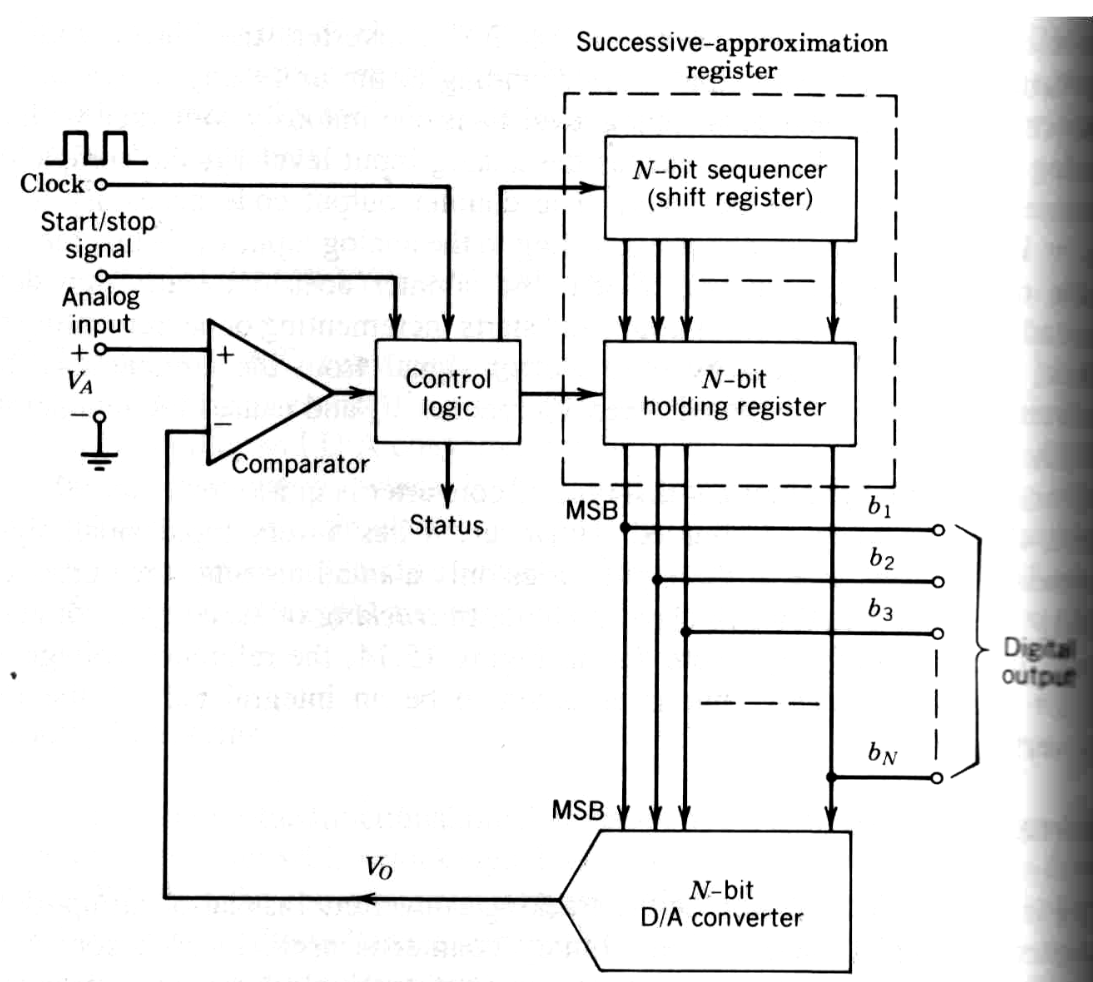
\includegraphics[width=0.8\linewidth]{microcontrollore/assets/ADC.png}
    \label{fig:ADC}
    \captionof{figure}{Schema di funzionamento dell'ADC}
\end{wrapfigure}

L'ADC ad approssimazioni successive per funzionare sfrutta un comparatore e un metodo di ricerca binaria. Attraverso una coversione Digitale-Analogica, il microcontrollore invia un segnale analogico al comparatore, il quale ritornerà un segnale positivo se il segnale inviato è maggiore di quello ricevuto, altrimenti ritornerà nullo.\\

Così facendo, il microcontrollore può ricavare con precisione e con poche iterazioni del metodo la rappresentazione binaria migliore per il valore analogico.\\

Altri aspetti positivi di questo metodo sono la presenza di un singolo compartore, il quale permette di diminuire notevolmente l'errore nella misura e la presenza di registri per la ricerca binaria, i quali rendono il processo più veloce di altri metodi.\\

\subsection{Programmazione}
Parte importante della programmazione con l'ADC è la calibrazione dell'apparato. Infatti, prima dell'utilizzo

\noindent
\begin{minted}[bgcolor = coding, linenos]{C}
    void ESPE_ADC_init(void){

	// azzeriamo per evitare casini di configurazione
	ADC3 -> SQR1 = 0;

	// ogni numero è collegato ad un pin a sèstante
	ADC3->SQR1 |= 0 <<ADC_SQR1_L_Pos;// ti dice quante misure deve prendere (n+1)
	ADC3->SQR1 |= 0 << ADC_SQR1_SQ1_Pos; // ti dice qual è la prima misura da fare

	ADC3->PCSEL |= ADC_PCSEL_PCSEL_0;//segna quali sono i canali in lettura per
                                        //velocità massima

	ADC3 -> CR &= ~ADC_CR_DEEPPWD_Pos;//Deep power down state
                                        //(se attivo non overclocka)
	ADC3 -> CR |= 1 << ADC_CR_ADVREGEN_Pos;//Voltage regulator activated

	ADC3 -> CR &= ~ADC_CR_ADCALDIF_Pos;//seleziona modalità differenziata
                                            //di calibrazione (a 0)
	ADC3 -> CR |= 1<< ADC_CR_ADCALLIN_Pos;//seleziona la modalità lineare
                                            //di calibrazione (a 1)
	ADC3 -> CR &= ~ADC_CR_ADEN_Pos;//Controlliamo che l'ADC non sia acceso e che
                                            //il bit sia stato resettato
	ADC3 -> CR |= 1<< ADC_CR_ADCAL_Pos;// Inizia la calibrazione

	while( ADC3->CR & ADC_CR_ADCAL ){							
            //Aspetti che la calibrazione sia finita, il bit viene cambiato dall'hardware
	}

	ADC3->ISR &= ~ADC_ISR_ADRDY_Pos;//Controlli che il bit per l'inizio della
                                        //presa dati sia a 0
	ADC3->CR |= 1<<ADC_CR_ADEN_Pos;//Attiviamo l'ADC (non la presa dati)
	while( !(ADC3->ISR & ADC_ISR_ADRDY)){						
            //Aspettiamo che sia setuppato correttamente
	}

	ADC3 -> IER |= ADC_IER_EOCIE;//Attiviamo l'interrupt

	ADC3 -> SMPR1 |= 0<<ADC_SMPR1_SMP0_Pos;
        //Possiamo aggiungere un ritardo di (n = 0) cicli prima della lettura

    }
\end{minted}
\label{code:ADC_init}

Oltre a impostare le misure da fare e il numero di misure che ogni ADC deve fare su ogni pin, all'interno della funzione è contenuto il processo di calibrazione dell'ADC. La calibrazione è fatta automaticamente dal microcontrollore usando dei valori di riferimento ma questo processo occupa tempo e, se non si aspettasse la fine della calibrazione per prendere la misura si avrebbero valori errati. Quindi c'è bisogno di un ciclo \textit{while()} per aspettare la fine della calibrazione.\\

La calibrazione è fatta accedendo a 2 Registri in particolare: il registro CR e il registro ISR. Il primo contiene i bit per la calibrazione e l'attivazione dell'ADC, mentre il secondo contiene i bit per controllare lo stato dell'ADC.\\

Una volta finita la calibrazione,  scrivendo
\noindent

\begin{minted}[bgcolor = coding]{C}
    ADC3-> CR |= ADC_CR_ADSTART
\end{minted}
l'ADC inizia a prendere le misure.\\
Per leggere i dati, invece, si può inserire nell'interrupt una funzione dedicata del tipo:

\noindent
\begin{minted}[bgcolor=coding , linenos]{C}

    #define len_vec 100
    uint_16 vec[len_vec];
    uint_8 counter_ADC = 0;
    uint_8 conversion_flag = 0;

    void ESPE_ADC_data(void){
        if( counter_ADC < len_vec){
            vec[counter_ADC] = ADC3->DR;
            counter_ADC++;
        }else{
            conversion_flag = 1;
            ADC3-> CR &= ~ADC_CR_ADSTART;
        }
    }

\end{minted}
\label{code:ADC_data}

In questo codice, il registro DR, il Data Register, contiene il valore misurato dall'ADC in Volt. Se il valore che si vuole non è in volt, è necessario fare una conversione. La conversione dipende da fattori come la tensione di riferimento dell'apparecchio che fa la misura e il valore massimo misurabile dall'ADC.\\

L'ultima riga, invece è necessaria per fermare l'ADC una volta che ha finito di prendere le misure.\\